\documentclass[a4paper,12pt,twoside]{article}
\usepackage[left=3cm,right=3cm,top=2cm,bottom=3cm]{geometry}
%\usepackage[square,authoryear,sort]{natbib}
\usepackage{url}
\usepackage{xcolor}
\usepackage{graphicx}
%\usepackage{pdfpages}
\usepackage{subcaption}
%\usepackage{pgfgantt}
%\usepackage{dirtytalk}

\makeatletter
\def\@makesectionhead#1{%
  \vspace*{50\p@}%
  {\parindent \z@ \raggedright \normalfont
    \interlinepenalty\@M
    \Huge\bfseries  \thesection.\quad #1\par\nobreak
    \vskip 40\p@
  }}
\makeatother

\makeatletter
\newcommand*{\toccontents}{\@starttoc{toc}}
\makeatother

\newtheorem{hypothesis}{Hypothesis}

\newtheorem{rquestion}{Research Question}


\let\endtitlepage\relax
\begin{document}

\title{\LARGE {\bf Semantic Modelling of Network Traffic for Anomaly Detection}\\
PhD 2\textsuperscript{nd} Year Progress Report
 \vspace*{-5mm}
}
\author{Henry Clausen}
%\date{October 2008}

\maketitle



\toccontents
%\begin{abstract}
%Text
%\end{abstract}


\section{Research progress in the last year}
  
\subsection{DetGen framework}
Building contextual models of network traffic means to build an understanding how different network interactions can be distinguished via their traffic trace. However, available network traffic datasets do not contain ground truth labels about the nature of computer interactions and often suffer from a lack of realism. To improve this and ensure that our models extract meaningful sets of sequences that represent these different interactions, we started developing a containerised traffic generation framework to generate traffic with ground truth labels. 



After focusing on the dynamic and scalable capabilities of DetGen suitable to train Machine Learning models in the ACSAC DYNAMICS last year, which has now finally been submitted to be published by the DYNAMICS organisers, I tried to emphasise the original design idea of DetGen more: The controlled and reproducible generation of traffic traces with ground truth information to understand how ML-models process specific network activities, which we call \textit{model probing}.

 
\begin{figure}
\centering
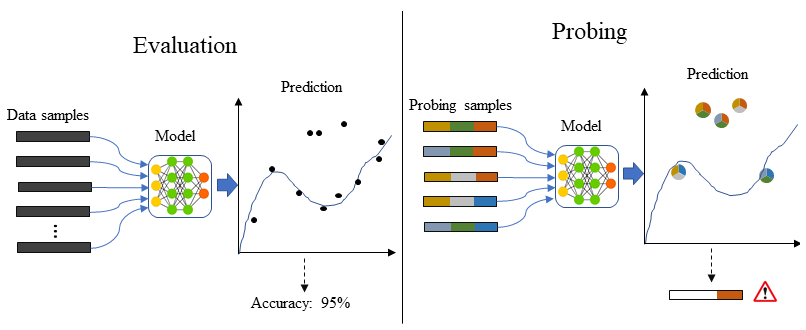
\includegraphics[width=\textwidth]{images/Eva_Prob.png}
\caption{Model evaluation and model probing with controlled data characteristics.}\label{Fig:Prob}
\end{figure}

For this, I examined how two state-of-the-art traffic classifiers could be probed, and performed several experiments to examine the control of DetGen over various traffic characteristics as well as the influence of these traffic characteristics on captured traffic traces with three novel traffic comparison metrics. The results from the probing of the classifiers were prepared into a paper and submitted and accepted at the \textit{Workshop on Traffic Measurements for Cybersecurity}, which is hosted at the \textit{S\&P}-conference in May. The examination of traffic determinism and their impact on traffic traces along with a detailed description of DetGen were submitted as a paper to the 2021 \textit{SecureComm} conference, for which we will receive acceptance notice on 17th May.


\subsection{Short-term contextual model of network flows using LSTM networks}\label{Sec:Short-term}

One of the main strains of work in year 1 and 2 of my PhD was focused on a building a LSTM-based neural network to capture meaningful sequences of \textit{NetFlows} and reflect reccurring patterns in a model. Learned contextual behaviour is reflected through the capability of the model to predict traffic protocols and network ports of flows in a session from a smaller subset of flows, with more accurate predictions being rewarded in the training process.

Despite the promising performance of this model, several submissions a paper to well-known conferences were unsuccessful and the paper was rejected mostly for a lack of novelty and scepticism of the real-world applicability. Last year, this work was finally accepted at the \textit{Machine Learning for Networking}-conference 2020. Some aspects that I improved for acceptance include:

\begin{enumerate}
\item I specified the scope of the model to the detection of U2R and R2L attacks, to which it is more suited than high volume attacks. I also exchanged the evaluation datasets to mutiple ones that are more suitable for this task and more realistic in nature.
\item I extended the model input features and model architecture to capture more complex sequences and decrease areas where the model was not performing well.
\item I replaced the CTU-14-dataset with the more suitable datasets CICIDS-17 and UGR-16, and identified suitable data traces for modelling and analysis. 
\item I focused more on the traffic structures the model is able to detect and explained the corresponding novelty of the model better. 
\item I included several state-of-the-art models as benchmark and also compared the now more complex model to a more shallow version to highlight how the learning of specific traffic structures was improved.
\end{enumerate}


\begin{figure}
\centering
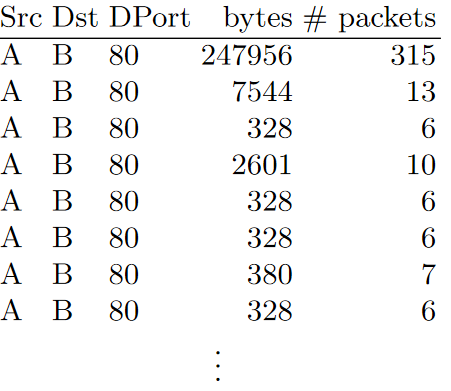
\includegraphics[width=0.4\textwidth]{images/traffic_sequence.png}
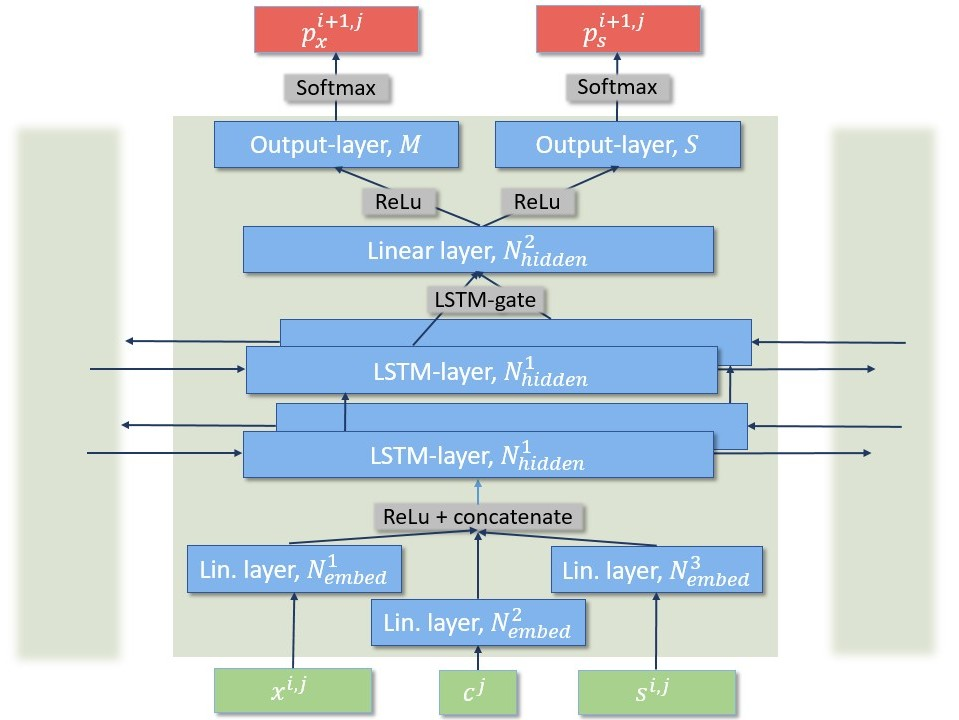
\includegraphics[width=0.49\textwidth]{images/LSTM_design_bi2.jpg}
\caption{Architectures of the model and corresponding traffic sequence of XSS-attack.}
\label{fig:LSTM}
\end{figure}


\subsection{Stepping stone detection}\label{Sec:BTstint}

%As part of my CASE PhD scholarship, I spent six weeks with my industrial sponsor at BT Labs Adastral Park in August and September 2019. Before starting this stint, I met with my industrial supervisors to define a project to work on that is both related to my PhD and is a relevant problem for BT. During this meeting, we agreed that the problem of detecting stepping stones was a suitable topic. 

In a stepping stone scenario, an attacker launches an attack not from their own computer but from intermediary hosts within an enterprise network that were previously compromised, often using an interactive relay session. A common approach in the literature to detect stepping stones is to identify correlation between two connections on a potential intermediary host. Attackers try to evade detection by inserting chaff packets and delays to make the connection appear uncorrelated. %Before starting this 6-week stint, I met with my industrial supervisors where we agreed that the problem of detecting stepping stones is of relevance for them and therefore a suitable topic for my time at BT Labs

The biggest challenge for this problem is that there are no available datasets available that describe stepping stone behaviour. Due to the success of the  DetGen framework, I started to implement several scenarios of interactive traffic relays using SSH-tunnels and netcat/netem for chaff and delay insertion. With this, I was able to generate significant amounts of traffic with a controllable amount of noise and delay to train and assess correlation models.

Since this problem in the described form turned out to not be relevant for BT anymore, I did not proceed to design my own detection method. 
I instead implemented 7 state-of-the-art methods for connection correlation and performed an extensive evaluation of their performance under various circumstances. The corresponding paper was submitted, accepted and published at the \textit{Network and Systems Security} conference 2020.


\begin{figure}
\centering
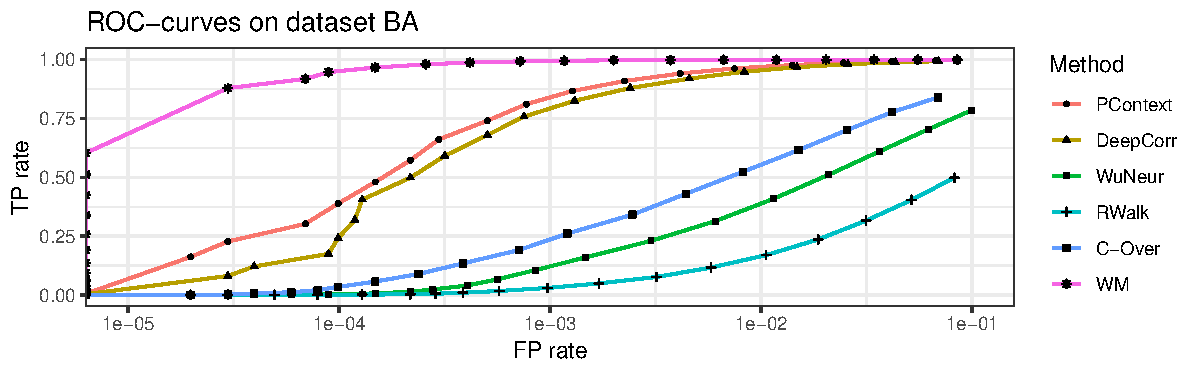
\includegraphics[width=0.9\textwidth]{images/Noevasion_4nodes-1.pdf}
\caption{Evaluation results on the generated data.}\label{stepstone}
\end{figure}

%After more consultation with a security expert, the scope of this project has been altered, which I describe in Section \ref{Bla}

%After finishing the stint at BT Labs, I continued to work on the traffic generation for a bit further before we had a call with Jake Hill, a security expert at BT. This call was meant to provide field knowledge to confirm and/or improve the data generation set-up. However, Jake stated that the problem of attackers launching attacks from intermediary hosts is after all not of great relevance for BT's operations. Instead, his notion of stepping stones described simple proxies relaying services (more on this in Section \ref{Sec:Relay}). In addition, further investigation suggests that the consensus in the literature is that connection correlation produces too many false positives and is not applicable in real-world scenarios. 




\section{Future plans}

\subsection{Challenges with publishing in Network Anomaly Detection and ACSAC conference}\label{Sec:Problems}

The original scope of this PhD-project was to built contextual models that represent software behaviour primarily from network traffic and potentially other external data sources, for adaptive anomaly intrusion detection.  
Over the course of the last year, it became clear that the successful publication of anomaly-based methods network intrusion detection methods is difficult today. This realisation was reflected during our unsuccessful attempts to publish the contextual network flow model described in Section \ref{Sec:Short-term} at the ACSAC and CODASPY conferences. Despite improving detection rates and false positive rates significantly on U2R and R2L on contemporary datasets, the main criticisms were a lack of novelty in terms of intrusion detection model and a general scepticism of real-world applicability. Prior attempts publication attempts by my supervisor and collaborating researchers yielded similar responses.

This is in line with conversations I had with senior researchers at the ACSAC conferences, who highlighted that anomaly-based methods have been applied to network traffic for over 15 years without convincing results. There seems to be a general scepticism of the detection capabilities and improvements that general-purpose anomaly-detection methods can provide in real-world scenarios due to high false-positive rates, in particular for network traffic. In the context of the proposed project, this raises doubt if research question 4 can be answered adequately for a PhD-project concerning general models of network behaviour. This also made us re-evaluate the scope of the project discussed in Section \ref{Sec:Encoder}.

General advice were to identify very specific applications for which taylored machine learning methods have the potential to yield good results. This is in line with the findings of Sommer and Paxson \cite{sommer_outside_2010} that anomaly detection methods should be "keeping the scope narrow" and providing an answer for "why the particular choice promises to perform well in the intended setting, considering domain-specific properties". "If one cannot make a solid argument for the relation of the features to the attacks of interest, the resulting study risks foundering on serious flaws."

\subsection{BT project}\label{Bla}

As part of my CASE PhD scholarship, I am spending 12 weeks in total with my industrial sponsor at BT Labs Adastral Park in the context of a student placement. While there, I am supposed to conduct research that is both relevant to my PhD-topic and to the operations of BT. Choosing a suitable topic is therefore not completely straightforward and could mean that the research conducted during the placement does not align completely with my PhD-topic.


In August and September 2019, I spent the first six weeks at Adastral Park. Before starting this stint, I met with my industrial supervisors to define a suitable project to work on. During this meeting, we agreed that the problem of detecting stepping stones was a suitable topic, as it was identified as a pressing issue for BT by their operational team, and could potentially benefit from from the developed DetGen framework described in Section \ref{Sec:BTstint} and the traffic sequence embedding techniques described in Section \ref{Sec:Encoder}.


After finishing the stint at BT Labs, I continued to work on the traffic generation for a bit further before we had a call with Jake Hill, a security expert at BT. This call was meant to provide field knowledge to confirm and/or improve the data generation set-up. However, Jake stated that the problem of attackers launching attacks from intermediary hosts is after all not of great relevance for BT's operations. Instead, his notion of stepping stones described simple proxies relaying services (more on this in Section \ref{Sec:Relay}). In addition, further investigation suggests that the consensus in the literature is that connection correlation produces too many false positives and is not applicable in real-world scenarios.

%\subsubsection{Scope of the project for publication}
With this information, I decided to scale this project down and produce a simple evaluation of existing connection correlation methods. Since the major contribution of this work so far is the large amount of detailed and varied data I can produce, this allows for the first time an independent assessment of existing methods. So far I have implemented and evaluated four different methods, and am in the process of finishing this project. I am currently producing a small paper from it, which I intend to publish at a smaller workshop or conference. 

\subsection{Submission of Stepping stone project and negotiation phase model}
%\section{Introduction and motivation}

With work being almost finished for the stepping stone project and the negotiation phase model also being well on the way, I am planning to write each project up into a paper for publication. Since the scope for each project was scaled back a bit, I am intending to submit them to smaller venues with a higher acceptance rate, and do not intend to spent more than three months completing both. A suitable venue for both might be the 2020 Conference on Machine Learning for Cyber Security.

\subsection{QUIC anomaly detection}

An advice I received at the ACSAC conference from Guofei Gu, the Program Chair, was to identify very specific and novel applications of machine learning methods to intrusion detection in order to produce publications that could be accepted at renowned venues. One such applications could be to the new transport layer QUIC. QUIC seeks to improve performance of connection-oriented web-applications using TCP. It is implemented on top of UDP and implements its own TCP-like packet control mechanisms. It allows for multiplexed HTTP-connections and resolves head-of-line blocking during packet loss as well as reducing latency by minimising round-trips during connection establishment. Furthermore, much of the QUIC implementation is moved from kernel to user space, which allows continuous updates of the protocol.

According to an NGINX-spokesperson, "since the protocol is new and things like stack optimization etc. still to catch up and since it's all user-space, there is a possibility to make changes to protocol very rapidly. This generates a higher attack surface than you would have over more layered approach with TCP and http on top." Initial investigations showed that there exists no research on mitigating intrusions over the QUIC protocol.%, which \textcolor{red}{...}

Due to the implementation in user-space, QUIC may introduce vulnerabilities that allow remote code execution on a host, such as in \textit{CVE-2017-15407} and \textit{CVE-2017-15398}. The detection of such code executions by building a combined model of QUIC packet exchanges and process starts/system calls therefore seems like a promising project that provides both novelty and relevance.

In particular, I believe the following conditions would allow for interesting results:
\begin{itemize}
\item Operation on a host (server or client) level
\item Combination of unencrypted packet packet stream and system calls/process starts corresponding
\item A sequential model that applies NLP-techniques to packet content and predicts probability of process start or particular system call (which could then correspond to code execution)
\item Traffic and system call/process log collection using a containerized framework.
\end{itemize}

In total, I would assign about six months work in this project to conclude.


One difficulty in this project is that there do not exist many identified vulnerabilities in the QUIC protocol yet, of which none are known to have been used in a successful attack. Therefore, it might be difficult to get enough malicious data for result validation. At this stage of my PhD, beginning a project that is not certain to be successful bears significant risk.  I am therefore currently spending a small amount of time reaching out to experts to verify that data for model validation is available and that the scope of this project is of relevance before fully committing to it.



\subsection{Service relay detection}\label{Sec:Relay}

As mentioned in Section \ref{Sec:BTstint}, disussion with a security expert at BT Labs indicated that the detection of simple proxy servers that relay protected services to third parties from the perspective of an ISP is a relevant and promising research project. Specific characteristics of this problem are:

\begin{itemize}
\item Unlike the original stepping stone problem, these relay proxies operate in a simplistic fashion and do not use evasion tactics. However, content can be forwarded using a different application or protocol than in the first connection.
\item Packets are sampled before observation, meaning that only every n-th packet for each connection is observed.
\item Benign proxies exist that can increase false-positives.
\end{itemize}

Initial investigations that I conducted showed that there are no publications yet that address this problem in any way, which indicates the potential for novel contributions. Since there exists no description or analysis of such proxies at all, this however also means that we are reliant on BT for knowledge and guidance on the problem definition and proxy operation mode. Also since no public dataset exists, we would have to implement and generate our own dataset and feedback with BT to check if it resembles the behaviour of such proxies. At the moment it seems that a suitable start would be to focus on video relay. Necessary steps for this project are:

\begin{itemize}

\item Implement a docker traffic generation scenario to generate realistic data, and parse them in a sampled manner.
\item start designing and implementing detection methods. As there are no evasion tactics involved, simple cumulative sum or moving window statistics with a p-value threshold seem like a good start.
\item Test these methods on the data with a suitable background of independent connections as well as benign proxies. Obtaining simple background data is not challenging, however we will have to discuss how and to what extend benign proxies should be included in the background data.
\item Evaluate and adjust/improve existing methods.

\end{itemize}

As we are reliant on the cooperation with BT Labs, we are not completely certain yet if this project will go ahead yet. Currently, they are retrieving data of service relay examples. We will have a further discussion with them later in April, which will bring more clarity. 

\subsection{Extension of Docker framework}\label{Sec:dockerext}

Due to very positive feedback at the workshop as well as encouragements and suggestions to extend the framework, Robert Flood and I are working further to extend the current traffic generation framework. The overall goal is to provide a tool that enables researchers to generate large data quantities of specific services of interest in arbitrary network configurations, complemented by multi-step attack scenarios in differing executions. This would be of specific interests to researchers who apply machine-learning techniques to specific network applications for which there is not sufficient realistic public data available.

Particular goals are:

\begin{enumerate}
\item Extend the framework to create datasets that resemble full fledged computer network with variable topology. For this, several subtasks need to be completed:

\begin{enumerate}

\item Embed all scenarios in a \textit{Mininet} framework in order to allow the fast inclusion of switches, routers, etc.

\item Build a mechanism that can generate variable or random network topologies.

\item Create a launch mechanism that starts and executes different traffic scenarios for a given network topology at times and locations drawn from appropriate distributions that resemble empirical network behaviour.

\end{enumerate}
\item Include the collection of application logs and system call logs for each container. These will then be matched with the corresponding traffic captures and receive the same ground truth labels.

\item Generate different multi-step attack executions on a set of network topologies to capture the similarities and disimilarities between different attack techniques and tactics.

\end{enumerate}

An advantage of this project is the pre-existing DetGen body, that is being extended here. This means that the timescale of the project depends on how many extensions should be implemented. It should be relatively easy to finish the project quikcly at any given time after about two months of work while having sufficient results to publish. 
%Since I am not the lead on this project, I currently do not have a timescale for its completion.


\section{Thesis plan}

In the light of the problems described in Section \ref{Sec:Problems} that we encountered in the field of anomaly-based intrusion detection, I believe that the scope of this PhD-project has to be altered slightly. As there will not be enough material directly concerning anomaly detection, the formulation of building anomaly-detection models describing software behaviour should be relaxed to general applications of ML (not just anomaly detection) in specific areas related to software defined behaviour. 
The overall unifying theme of this PhD so far has been centered around small-scale traffic structures generated by software-defined computer interactions and applications of ML language models to it, in other words \textbf{Modelling computer interactions as a language}.
This could be based of the reoccurring use of traffic (and potentially system/program logs) generation for machine learning. The generated traffic could then be verified as valuable by the implemented intrusion detection applications.

All applications implemented so far except for the flow-level model are driven (in part) by our traffic generation:
\begin{itemize}
\item Flow-level LSTM model

\item stepping stone detection
\item traffic relay
\item LSTM encoder
\item QUIC anomaly detection
\end{itemize}

Overall, all these applications except for the traffic relay detection are concerned with software-defined fine-grained structures. Below, I outline the different chapters that I believe should be included in my thesis:

\begin{enumerate}


\item Introduction and related work

This chapter could largely draw from the existing introduction in the research proposal as well as the extensive literature survey I conducted. Updates on the scope as well as recent developments in related work would have to be added. %This should take less then three weeks.

\item Background: Anomaly detection and challenges in security

This chapter outlines the motivation to use anomaly-based detection models instead of classification-based ones. It furthermore highlights why anomaly detection is more difficult in security than in other areas, and what currently prevents it from being deployed outside of academia.

\item Background: Language models and their application to security

This chapter briefly outlines different techniques used in language modelling,  and how they can be used to build data representation useful for anomaly-detection. It also discusses previous applications of language models in security.

\item Data sources, datasets, and data generation with realistic small scale structures

This chapter will draw largely on the work conducted for the DetGen traffic generation framework.

\item Computer communication structures and the effect of malicious behaviour on them

This chapter will describe the different structures that the different layers of software-defined communication can have on the collected data. These descriptions and their corroboration can be taken from work in each of the projects described above. Furthermore, this chapter will describe how attacks can alter these structures due to the distinct approach they are taking, and why it is worth building models that focus on small-scale traffic structures.

\item Traffic as a language and detection models

This chapter will describe how network traffic can be described by a language model, and how to construct anomaly-based models from it. The chapter will then proceed to describe the different approaches I worked on and their respective results:

\begin{enumerate}

\item Flow-based modelling

\item Connection setup model

\item Traffic relating to process initialisations in the QUIC protocol

\item Detecting similarity in computer connections


\end{enumerate}

\item Conclusions

\end{enumerate}

\subsection{Thesis completion plan}

\begin{enumerate}

\item month
\begin{itemize}
\item Finish stepping stone project
\item Inquire about the prospect of QUIC project
\item Discuss with BT the boundary conditions and data sources for a service relay problem 
\end{itemize}

\item month
\begin{itemize}
\item Work on connection setup project
\item Start producing paper from connection setup project
\item Finish inquiry about the prospect of QUIC project
\end{itemize}

\item month
\begin{itemize}
\item Finish connection setup project
\item Start developing anomaly-detection model for QUIC project
\end{itemize}

\item month
\begin{itemize}
\item Continue development of model for QUIC project
\item Work on dataset for QUIC project
\end{itemize}

\item month
\begin{itemize}
\item Work on dataset for QUIC project
\item Gather data representing malicious QUIC traffic
\end{itemize}

\item month
\begin{itemize}
\item Evaluate and tune results for QUIC project
\item Start producing paper for QUIC project
\end{itemize}

\item month
\begin{itemize}
\item Finish paper for QUIC project
\item Work on data generation for service relay project
\end{itemize}

\item month
\begin{itemize}
\item Begin 2. stint at BT
\item Work on model for service relay project
\end{itemize}

\item month
\begin{itemize}
\item Finish 2. stint at BT
\item Evaluate model for service relay project
\end{itemize}

\item month
\begin{itemize}
\item Discuss further steps in service relay project, potentially produce paper
\item Extend DetGen framework
\end{itemize}

\item month
\begin{itemize}
\item Extend DetGen framework
\end{itemize}

\item month
\begin{itemize}
\item Extend DetGen framework
\item Produce paper for DetGen framework
\end{itemize}


\textbf{Thesis write-up}

\item month
\begin{itemize}
\item Revise literature review
\item Complete chapter 1 and 2
\item Compile a map of different language models for chapter 3
\end{itemize}
\item month
\begin{itemize}
\item Complete chapter 3
\item Assess the requirements for chapter 4 and compare to results of DetGen project
\item Start working on chapter 4
\end{itemize}

\item month
\begin{itemize}
\item Complete chapter 4
\item Compile a map of different traffic structures observed in each project
\item Compile a map of different attacks and their effect on respective structures
\item Start chapter 5

\end{itemize}
\item month
\begin{itemize}
\item Complete chapter 5
\item Assess the results of each project, and decide order and weight of each project on chapter 6
\item Decide if anything is needed as input for chapter 6
\item Start chapter 6
\end{itemize}

\item month
\begin{itemize}
\item Complete chapter 6
\end{itemize}
\end{enumerate}



%\addcontentsline{toc}{section}{Bibliography}
\bibliographystyle{abbrv}
\bibliography{refs}

\end{document}